\level{1}{Tracker} \label{sec:tracker}

Tracker è l'applicazione web sviluppata da \groupname{}, disponibile all'indirizzo \insuri{http://kaizenteam.it/tracker/}, che consente di automatizzare il tracciamento dei requisiti durante l’avanzamento del progetto. \\
L'applicativo è in grado di fornire le seguenti funzioni:
\begin{itemize}
	\item aggiunta di fonti;
	\item aggiunta di requisiti;
	\item associazione tra fonti e requisiti;
	\item storico delle modifiche;
	\item tracciamento fonti-requisiti;
	\item tracciamento requisiti-fonti;
	\item tracciamento delle tipologie degli errori rilevati in fase di verifica.
\end{itemize}

Per agevolare la stesura del documento di \insdoc{Analisi dei Requisiti}, è stata aggiunta una funzionalità che permette l’esportazione automatica dei requisiti in \LaTeX, comprensivi di tracciamento fonti-requisiti e requisiti-fonti. Il \insfile{Makefile} è capace di scaricare autonomamente i sorgenti \LaTeX{} e di inserirli all’interno della documentazione. \\
Seguono alcune schermate dell’interfaccia:

\begin{figure}[H]
	\centering
	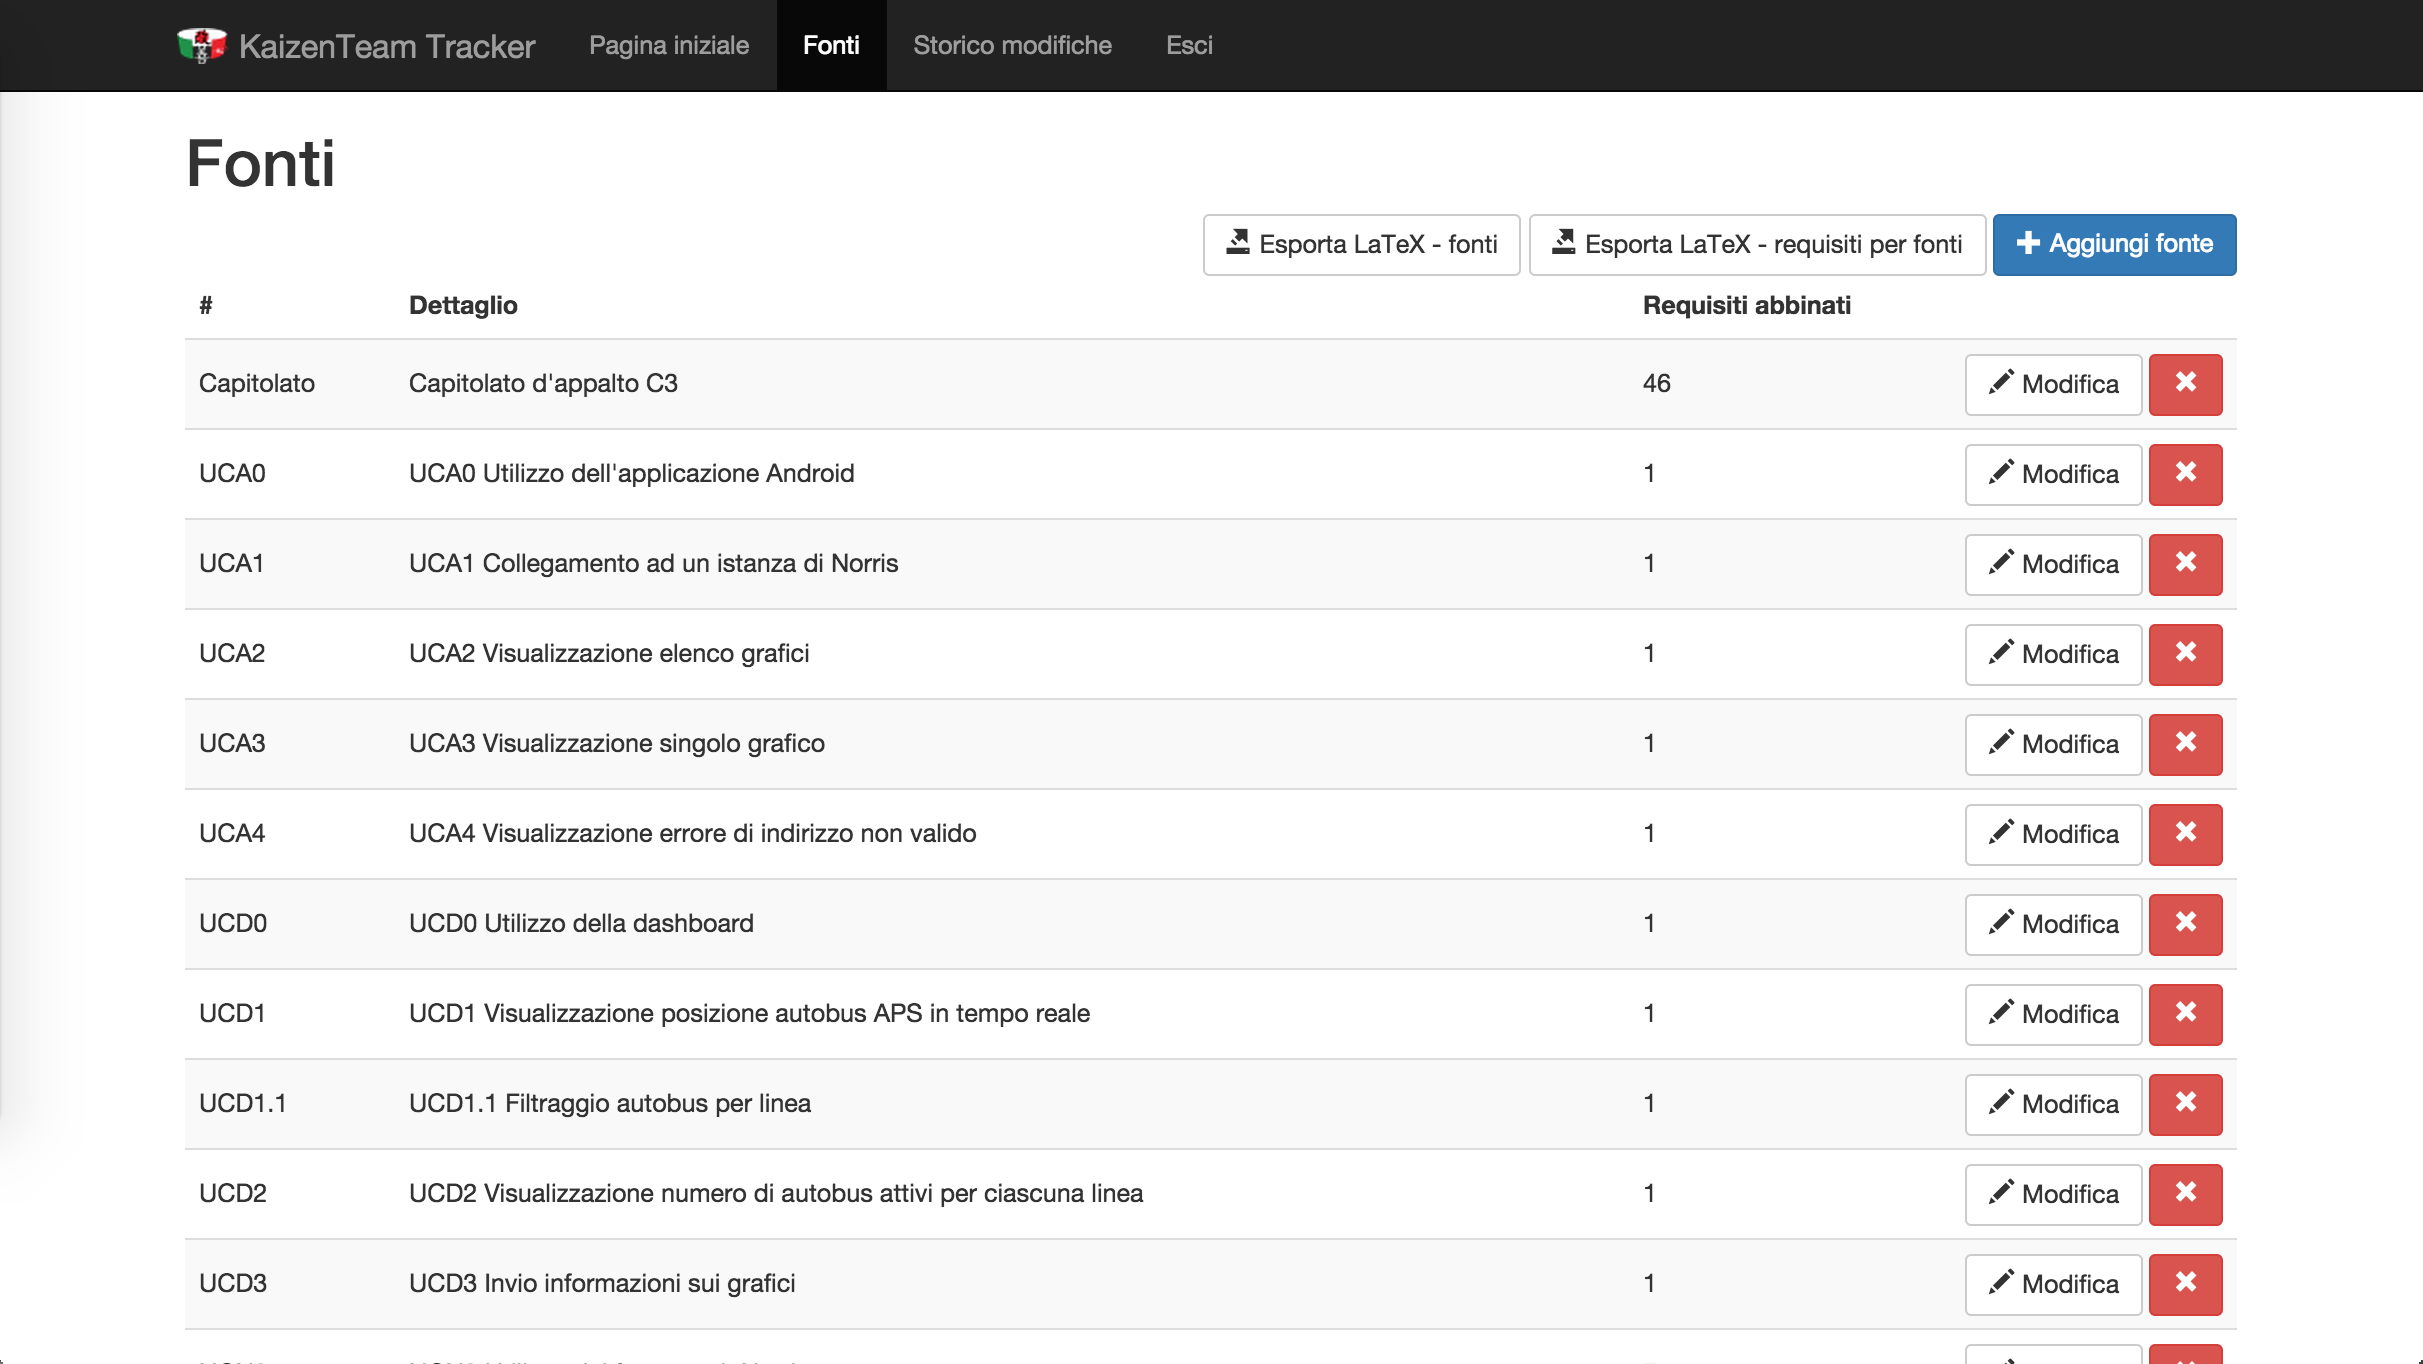
\includegraphics[width=\textwidth]{Pics/TrackerFonti}
	\caption{Tracker - Aggiunta delle fonti}
\end{figure}


\begin{figure}[H]
	\centering
	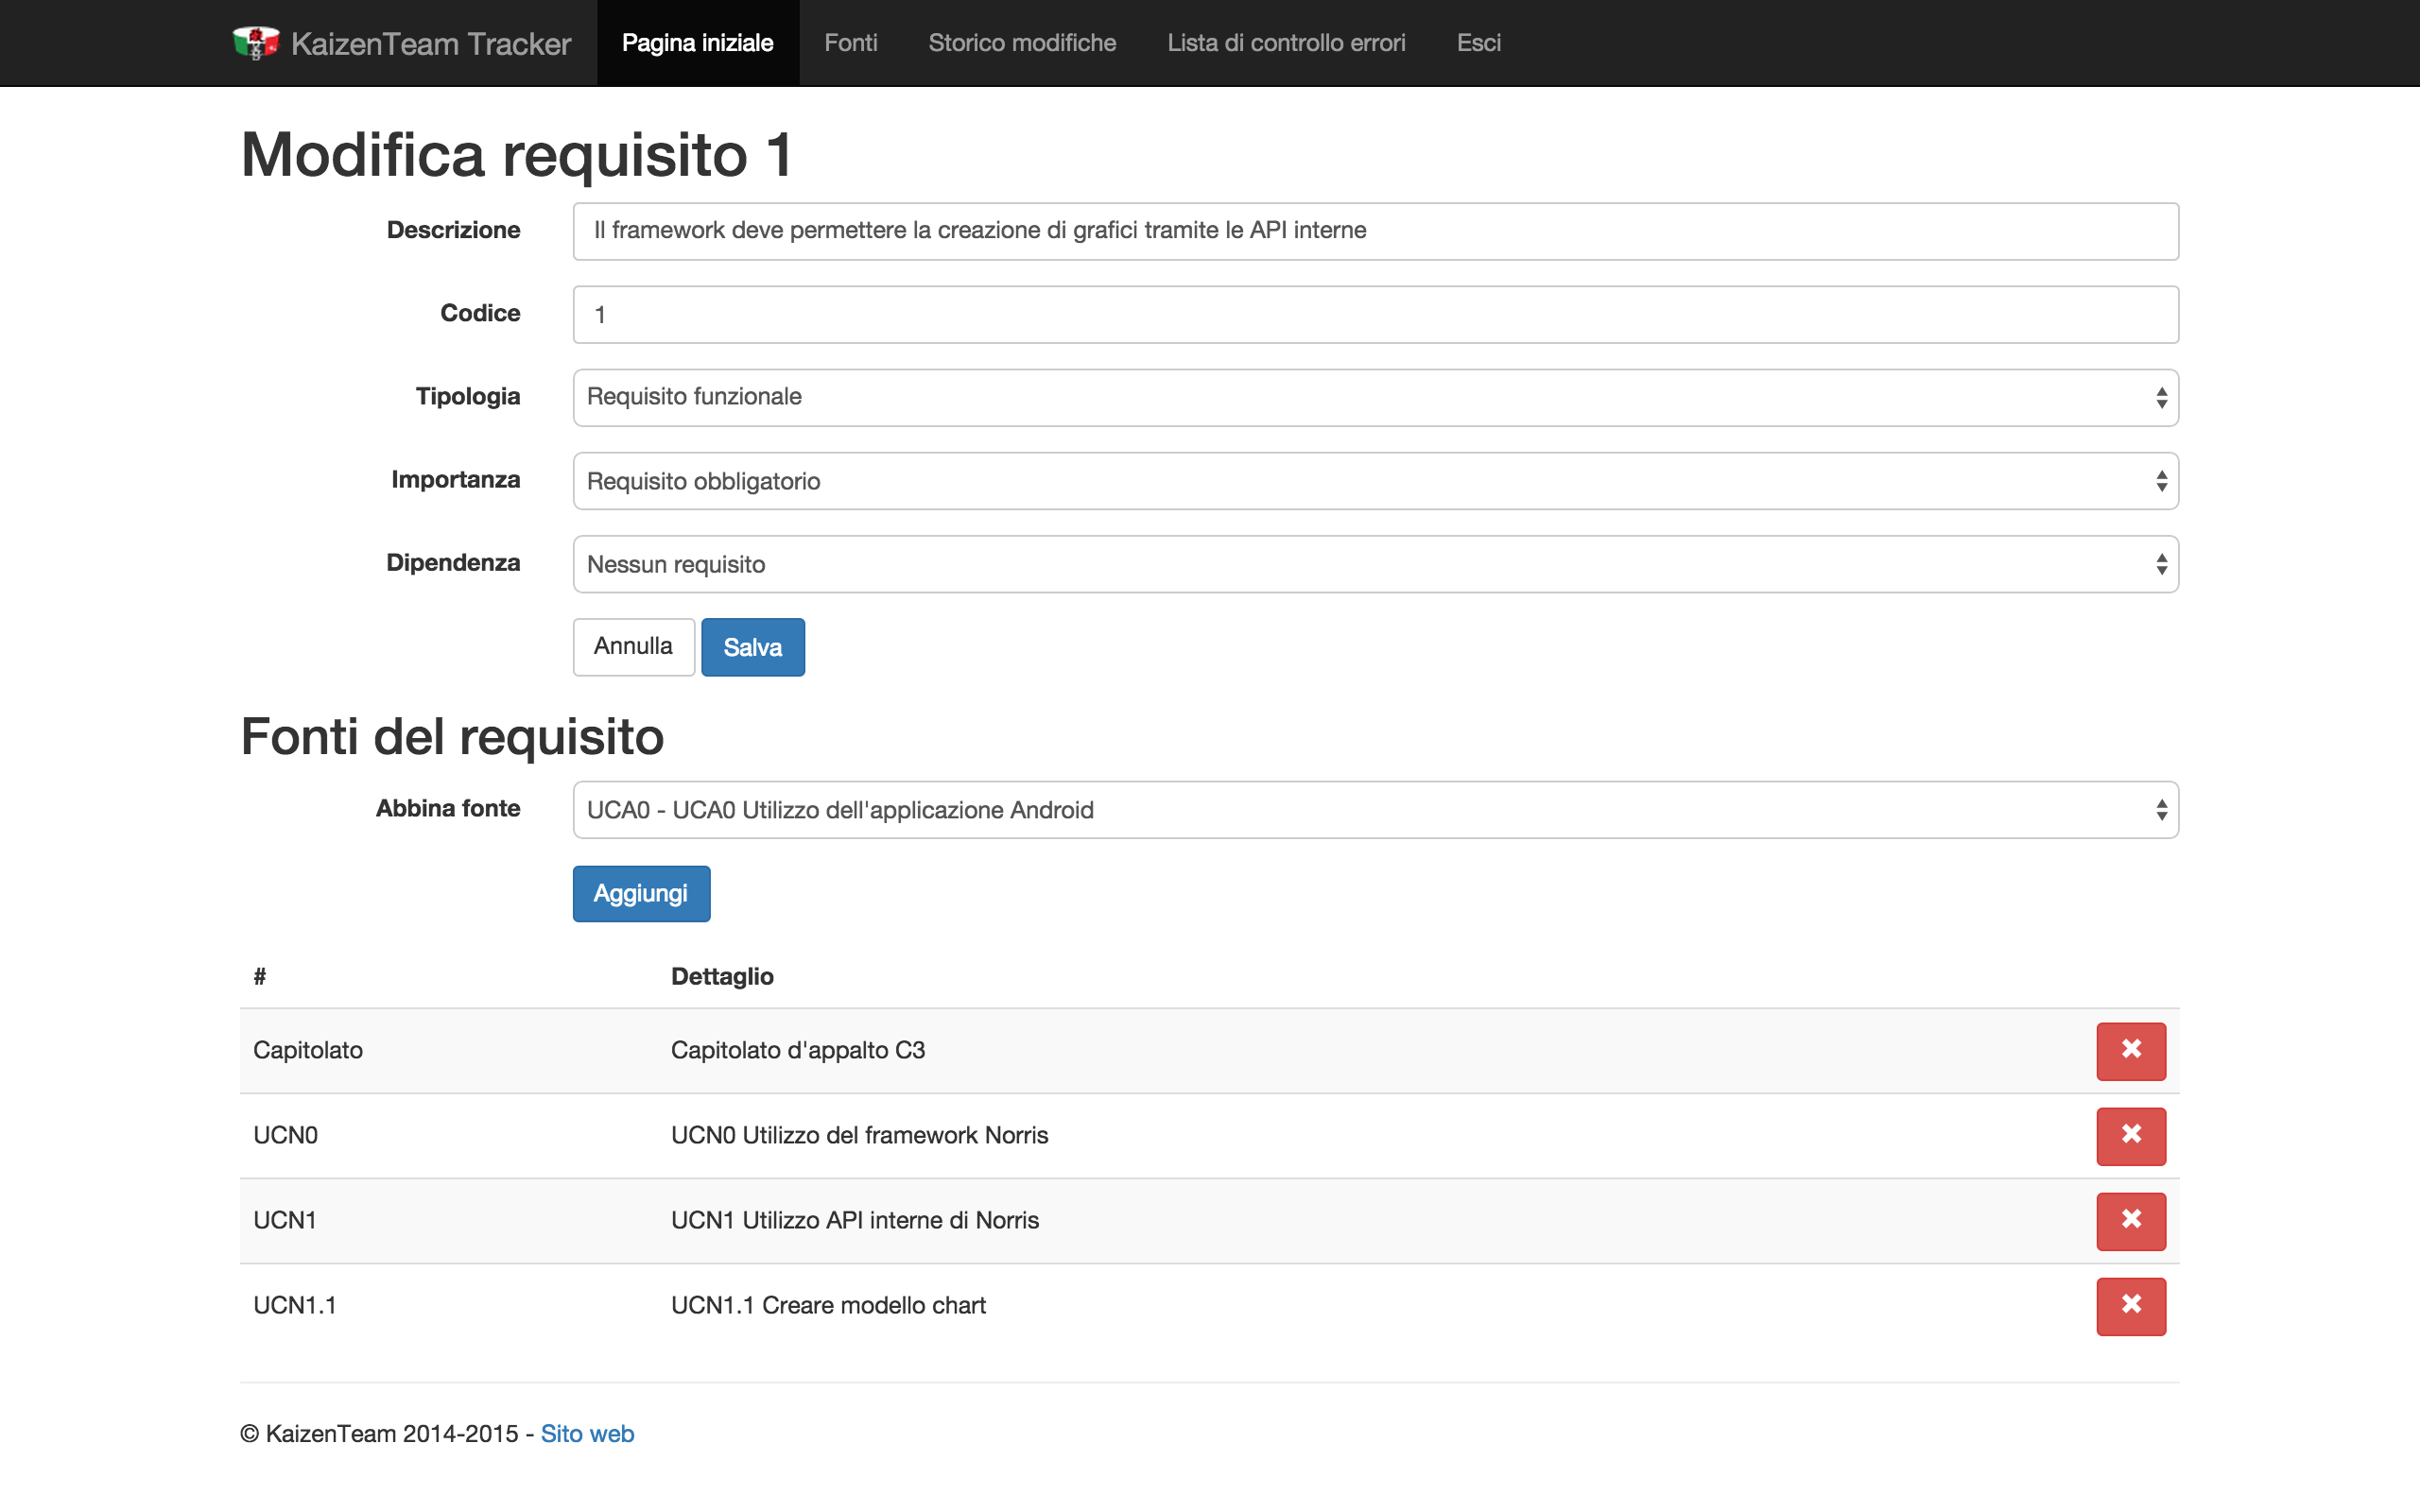
\includegraphics[width=\textwidth]{Pics/TrackerModificaRequisito}
	\caption{Tracker - Modifica di un requisito}
\end{figure}
